% =========================================================
% TP5 -- Calibracion de una capa de elusion con trayectorias experimentales
% Presentacion de referencia (entregable b). Formato segun la guia de
% presentaciones de la catedra (../tp-2/GuiaPresentaciones.pdf, fuera de este
% repositorio) y las devoluciones recogidas en FEEDBACK.md (TP2, TP3 y TP4):
%   * sin diapositiva de contenido ni caratulas de bloque: solo separadores
%   * poco detalle al inicio; cada concepto se explica UNA vez donde hace falta
%   * nada aparece sin estar definido antes: ningun termino se usa sin haberlo
%     dicho (devolucion del TP4 sobre "solucion algebraica" y "celda de indice")
%   * lo importante ocupa la pantalla: figura grande, texto minimo
%   * tabla de parametros en bloques, con las unidades en un solo lugar
%   * UML solo del motor de simulacion
%   * nombres de eje en una sola linea, con la unidad y coma decimal; leyenda
%     adentro sin tapar datos; ningun eje con valores equiespaciados que no lo
%     sean (devolucion del TP4, D24)
%   * cada diapositiva de figura es el grafico grande mas dos o tres vinetas
%   * conclusiones como punteo corto, solo con cifras de las figuras mostradas,
%     y sin tener que volver atras para mostrarlas
%   * los links a YouTube van en el PDF que se entrega, y los videos quedan
%     PUBLICOS (devolucion del TP4: "las animaciones no se pueden ver")
% y el enunciado del TP5:
%   * a la descripcion matematica de la capa de elusion se le dedica MAS tiempo
%     que a la introduccion matematica habitual: son tres diapositivas (4, 5
%     y 6), con el esquema de la deteccion, el del target temporal y los casos
%     limite.
%
% Las figuras se leen de slides-images/ (make slides-images), numeradas con la
% diapositiva en la que van. Los esquemas TikZ y la tabla de parametros se
% escriben en LaTeX con \input{figuras/*.tikz} y make slides-images-tikz los
% renderiza ademas a PNG, asi que en slides-images/ esta TODA imagen de la
% charla: es la carpeta con la que se arma la presentacion a mano.
%
%   make documentos        -> report/build/presentacion.pdf
% =========================================================

\documentclass[aspectratio=169,11pt]{beamer}

\usepackage[utf8]{inputenc}
\usepackage[T1]{fontenc}
\usepackage[spanish,es-noquoting,es-noshorthands]{babel}

\usepackage{amsmath}
\usepackage{amssymb}
\usepackage{graphicx}
\usepackage{booktabs}
\usepackage{siunitx}
\sisetup{output-decimal-marker={,}, per-mode=symbol}
\usepackage{tikz}
\usetikzlibrary{arrows.meta,positioning,fit,backgrounds,calc,shapes.multipart}

% ---------------------------------------------------------
% Tema (el mismo del TP3 y el TP4). Colores y atajos en comun.tex, compartidos
% con los esquemas TikZ de figuras/.
% ---------------------------------------------------------

% Colores y atajos compartidos por presentacion.tex y por figuras/render.tex
% (los esquemas TikZ de las diapositivas, renderizados sueltos a slides-images/).

\definecolor{azul}{RGB}{23,66,110}
\definecolor{acento}{RGB}{197,90,17}
\definecolor{gris}{RGB}{110,118,128}
\definecolor{grisclaro}{RGB}{236,238,241}
\definecolor{izquierda}{RGB}{31,95,191}
\definecolor{derecha}{RGB}{214,39,40}
\definecolor{target}{RGB}{44,160,44}
\definecolor{medida}{RGB}{110,118,128}

% La capa de elusion y sus dos parametros.
\newcommand{\ta}{\ensuremath{t_a}}
\newcommand{\ds}{\ensuremath{d_s}}
\newcommand{\tdca}{\ensuremath{\tau^{*}}}
\newcommand{\ddca}{\ensuremath{d^{*}}}
\newcommand{\Dreq}{\ensuremath{D}}

% Vectores y operadores.
\newcommand{\vr}{\ensuremath{\mathbf{r}}}
\newcommand{\vv}{\ensuremath{\mathbf{v}}}
\newcommand{\vF}{\ensuremath{\mathbf{F}}}
\newcommand{\vq}{\ensuremath{\mathbf{q}}}
\newcommand{\vT}{\ensuremath{\mathbf{T}}}
\newcommand{\ehat}{\ensuremath{\hat{\mathbf{e}}}}
\newcommand{\nhat}{\ensuremath{\hat{\mathbf{n}}}}
\newcommand{\that}{\ensuremath{\hat{\mathbf{t}}}}
\newcommand{\shat}{\ensuremath{\hat{\mathbf{s}}}}
\newcommand{\dtexp}{\ensuremath{\Delta t_{\text{exp}}}}
\newcommand{\dt}{\ensuremath{\Delta t}}

% Las dos metricas del enunciado.
\newcommand{\Euno}{\ensuremath{E^{(1)}}}
\newcommand{\Edos}{\ensuremath{E^{(2)}}}
\newcommand{\mEuno}{\ensuremath{\langle E^{(1)}\rangle}}
\newcommand{\mEdos}{\ensuremath{\langle E^{(2)}\rangle}}

\newcommand{\cita}[1]{{\scriptsize\color{gris}(#1)}}
\newcommand{\rotulo}[1]{{\color{azul}\bfseries #1}}


\usetheme{default}
\usecolortheme{default}
\setbeamertemplate{navigation symbols}{}
\setbeamercolor{structure}{fg=azul}
\setbeamercolor{frametitle}{fg=azul}
\setbeamercolor{title}{fg=azul}
\setbeamercolor{alerted text}{fg=acento}
\setbeamerfont{frametitle}{size=\large,series=\bfseries}
\setbeamerfont{title}{size=\LARGE,series=\bfseries}
\setbeamertemplate{itemize item}{\color{azul}\rule[0.25ex]{0.5ex}{0.5ex}}
\setbeamertemplate{itemize subitem}{\color{gris}\rule[0.25ex]{0.4ex}{0.4ex}}
\setbeamersize{text margin left=0.6cm, text margin right=0.6cm}

\setbeamertemplate{frametitle}{%
    \vspace*{0.35em}%
    \hspace*{0.6cm}%
    \parbox{\dimexpr\linewidth-0.6cm\relax}{\raggedright
        \usebeamerfont{frametitle}\usebeamercolor[fg]{frametitle}\insertframetitle\par
        \vspace{-0.25em}\textcolor{azul!30}{\rule{\linewidth}{0.9pt}}}%
}

\setbeamertemplate{footline}{%
    \hbox{%
    \begin{beamercolorbox}[wd=\paperwidth,ht=2.0ex,dp=1.2ex,leftskip=0.6cm,rightskip=0.6cm]{}%
        {\scriptsize\color{gris}%
         Calibración de una capa de elusión\hfill Grupo 10 -- Comisión S2\hfill\insertframenumber}%
    \end{beamercolorbox}}%
}

% ---------------------------------------------------------
% Atajos
% ---------------------------------------------------------

% Link a la animacion, debajo del cuadro fijo. En la version en vivo esta
% diapositiva se proyecta con el video embebido y sin link (D12 del TP2).
\newcommand{\video}[1]{{\tiny\href{#1}{\texttt{\detokenize{#1}}}}}

% Figura principal a la izquierda y dos o tres vinetas cortas a la derecha.
\newcommand{\figbul}[2]{%
    \vspace{-0.2em}
    \begin{columns}[c,onlytextwidth]
        \begin{column}{0.60\textwidth}
            \centering
            \includegraphics[width=\linewidth,height=0.76\textheight,keepaspectratio]{#1}
        \end{column}\hfill
        \begin{column}{0.37\textwidth}
            \small
            \begin{itemize}\setlength{\itemsep}{0.5em}
                #2
            \end{itemize}
        \end{column}
    \end{columns}}

\newcommand{\figbulw}[3][0.4em]{%
    \vspace{-0.2em}
    \begin{columns}[c,onlytextwidth]
        \begin{column}{0.55\textwidth}
            \centering
            \includegraphics[width=\linewidth,height=0.72\textheight,keepaspectratio]{#2}
        \end{column}\hfill
        \begin{column}{0.43\textwidth}
            \small
            \begin{itemize}\setlength{\itemsep}{#1}
                #3
            \end{itemize}
        \end{column}
    \end{columns}}

% El recinto es largo y bajo: las figuras del plano x-y y los cuadros de
% animacion van a lo ancho de la diapositiva, con las vinetas debajo en dos
% columnas.
\newcommand{\figancha}[3][0.90]{%
    \vspace{-0.4em}
    \begin{center}
        \includegraphics[width=#1\textwidth,height=0.46\textheight,keepaspectratio]{#2}
    \end{center}
    \vspace{-0.3em}
    {\footnotesize\begin{columns}[t,onlytextwidth]#3\end{columns}}}

\newcommand{\colvin}[2][0.48]{%
    \begin{column}{#1\textwidth}
        \begin{itemize}\setlength{\itemsep}{0.35em}#2\end{itemize}
    \end{column}}

% La ultima vineta de cada figura: los parametros fijos bajo los que se
% obtuvo (GuiaPresentaciones 1.7, "descriptas al costado de la figura").
\newcommand{\cond}[1]{\item {\scriptsize\color{gris} #1}}

\graphicspath{{../slides-images/}}

\title{Calibración de una capa de elusión}
\subtitle{Trayectorias experimentales de peatones que se cruzan de frente}

\begin{document}

% =========================================================
\begin{frame}[plain,noframenumbering]
    \vfill
    \begin{center}
        {\usebeamerfont{title}\usebeamercolor[fg]{title}\inserttitle}\\[0.3em]
        {\large\color{gris}\insertsubtitle}\\[1.0em]
        \textcolor{azul!30}{\rule{0.45\textwidth}{1pt}}\\[1.0em]
        {\small
        \begin{tabular}{ccc}
            Javier Liu & Juan Ignacio Cantarella & Nicolás Rivas \\[0.15em]
            {\footnotesize\color{gris}64332} &
            {\footnotesize\color{gris}64509} &
            {\footnotesize\color{gris}64292}
        \end{tabular}}\\[1.4em]
        {\footnotesize Instituto Tecnológico de Buenos Aires \quad\textbar\quad Simulación de Sistemas}\\[0.3em]
        {\footnotesize\color{gris} Trabajo Práctico 5 \enspace\textbar\enspace Problema 1 \enspace\textbar\enspace Grupo 10 -- Comisión S2 \enspace\textbar\enspace 2026 Q2}
    \end{center}
    \vfill
\end{frame}

\AtBeginSection[]{%
    \begin{frame}
        \vfill
        \begin{center}
            {\Large\bfseries\color{azul}\insertsectionhead}\\[0.5em]
            \textcolor{azul!30}{\rule{0.28\textwidth}{1pt}}
        \end{center}
        \vfill
    \end{frame}}

% =========================================================
\section{Introducción}
% =========================================================

\begin{frame}{El experimento: elusión 1 contra 1 de frente}
    \vspace{-0.3em}
    \begin{columns}[c,onlytextwidth]
        \begin{column}{0.46\textwidth}
            \small
            \begin{itemize}\setlength{\itemsep}{0.65em}
                \item En cada prueba sale una persona de la \textcolor{izquierda}{\textbf{fila
                      izquierda}} y otra de la \textcolor{derecha}{\textbf{fila derecha}} y
                      se cruzan de frente en $y \approx \SI{2}{\meter}$.
                \item La cátedra da las dos trayectorias medidas,
                      $\vr_i^{\text{exp}}(t_k)$ con $t_k = k\,\dtexp$ y
                      $\dtexp = \SI{66.58}{\milli\second}$:
                      $M = 19$ eventos, 38 peatones, \num{2543} instantes.
                \item Pasan a $d_{\min}$ entre $0{,}49$ y \SI{0.92}{\meter}:
                      se eluden \textbf{sin tocarse} ($2r = \SI{0.5}{\meter}$).
                \item Hay que proponer y calibrar una capa de elusión de
                      \textbf{dos parámetros}.
            \end{itemize}
        \end{column}\hfill
        \begin{column}{0.52\textwidth}
            \centering
            \resizebox{\linewidth}{!}{% El experimento de la catedra: dos filas de personas, una a la izquierda y
% otra abajo a la derecha. En cada prueba sale una de cada fila y las dos se
% cruzan de frente alrededor de y = 2 m. De cada prueba la catedra da las dos
% trayectorias medidas a 15 cuadros por segundo.
\begin{tikzpicture}[scale=0.82, >={Stealth[length=2.2mm]}, font=\footnotesize]
  % Area de seguimiento
  \draw[rounded corners=2pt, fill=grisclaro, draw=gris]
        (0,-0.6) rectangle (11,4.0);
  \node[gris, anchor=north east] at (11,4.0) {área de seguimiento};

  % Fila izquierda
  \foreach \k in {0,1,2} {
    \fill[izquierda!35] (0.7,-0.2-0.55*\k) circle (0.2);
  }
  \node[izquierda, anchor=north] at (0.7,-0.75-1.1) {fila izquierda};

  % Fila derecha (abajo a la derecha)
  \foreach \k in {0,1,2} {
    \fill[derecha!35] (8.1,-0.2-0.55*\k) circle (0.2);
  }
  \node[derecha, anchor=north] at (8.1,-0.75-1.1) {fila derecha};

  % Las dos trayectorias de una prueba
  \draw[izquierda, very thick, ->]
        (0.7,0.3) .. controls (1.2,1.6) and (2.6,1.8) .. (4.0,1.72)
        .. controls (6.0,1.62) and (8.0,1.95) .. (10.3,2.1);
  \draw[derecha, very thick, ->]
        (8.1,0.3) .. controls (8.4,1.5) and (7.2,2.1) .. (5.6,2.28)
        .. controls (4.2,2.44) and (2.0,2.2) .. (0.4,2.08);

  % Discos en el cruce
  \fill[izquierda] (4.55,1.56) circle (0.26);
  \fill[derecha]   (4.55,2.52) circle (0.26);
  \draw[<->, thick] (4.55,1.82) -- (4.55,2.26)
        node[midway, right=3pt, black] {$d_{\min}$};
  \node[anchor=south, black] at (4.55,2.86) {cruce, $y \approx \SI{2}{\meter}$};

  % Ejes
  \draw[->, gris] (0,-0.6) -- (0,4.0) node[anchor=south east] {$y$};
  \draw[->, gris] (0,-0.6) -- (11,-0.6) node[anchor=north east] {$x$};
\end{tikzpicture}
}
        \end{column}
    \end{columns}
\end{frame}

\begin{frame}{Los datos: las 19 pruebas medidas}
    \figbulw[0.5em]{slide-03-eventos-trayectorias.png}{%
        \item Las 38 trayectorias, cada una del primer al último cuadro de su
              prueba. Las dos filas se ven como los racimos verticales en
              $x \approx 0{,}7$ y \SI{8.1}{\meter}.
        \item El arco de elusión es \textbf{sistemático}: quien sale por la
              izquierda baja a $y \approx 1{,}6$--$1{,}8$ y quien sale por la
              derecha sube a $2{,}2$--\SI{2.7}{\meter}.
        \item \alert{En 14 de los 19 cruces cada uno pasó por su derecha}; en los
              otros 5, al revés. No hay una convención estricta, y eso después
              aparece en el error que le queda al modelo.
        \cond{las 19 pruebas superpuestas; una línea por peatón}
    }
\end{frame}

\begin{frame}{Modelo: SFM sin fuerza social}
    \vspace{-0.3em}
    \small
    \setlength{\abovedisplayskip}{5pt}\setlength{\belowdisplayskip}{5pt}
    Newton para cada agente, con el \textbf{término de conducción} hacia su target y el
    \textbf{contacto} granular de Helbing, Farkas y Vicsek (2000) \cita{sin el término social
    $A\,e^{(r_{ij}-d_{ij})/B}$}:
    \[
        m\,\frac{d\vv_i}{dt}
        = \underbrace{\frac{m}{\tau}\left(v_i^{d}\,\ehat_i^{\,d} - \vv_i\right)}_{\text{conducción}}
        + \underbrace{\sum_{j \ne i}\Big[k\,\xi_{ij}\,\nhat_{ij}
          + \kappa\,\xi_{ij}\,(\Delta\vv_{ji}\cdot\that_{ij})\,\that_{ij}\Big]}_{\text{contacto, sólo si } \xi_{ij} > 0}
    \]
    con $\xi_{ij} = r_i + r_j - d_{ij}$ el solapamiento,
    $\nhat_{ij} = (\vr_i - \vr_j)/d_{ij}$, $\that_{ij}$ su perpendicular y
    $\Delta\vv_{ji} = \vv_j - \vv_i$.
    \vspace{0.6em}

    \begin{itemize}\setlength{\itemsep}{0.45em}
        \item \alert{El modelo no anticipa}: mientras no hay solapamiento, el
              agente va derecho a su target y la única señal del otro llega
              cuando ya lo está tocando.
        \item Lo único que decide a dónde va es $\ehat_i^{\,d}$, la dirección de
              la velocidad deseada. \textbf{La capa de elusión actúa ahí y en
              ningún otro lado}: no agrega fuerzas ni cambia las reglas del
              modelo.
        \item El agente \textbf{se detiene al llegar} a su target final (a menos
              de un radio): ahí $v_i^{d} = 0$ y la conducción lo frena en $\tau$.
    \end{itemize}
\end{frame}

\begin{frame}{Capa de elusión (1/3): detección del conflicto}
    \vspace{-0.2em}
    \begin{columns}[c,onlytextwidth]
        \begin{column}{0.56\textwidth}
            \centering
            \resizebox{\linewidth}{!}{% Capa de elusion, paso 1: deteccion del conflicto por extrapolacion lineal.
% Con Dr = r_j - r_i y Dv = v_j - v_i, el instante de minima aproximacion es
% tau* = -(Dr . Dv)/|Dv|^2 y la separacion predicha ahi, d* = |Dr + Dv tau*|.
% Hay conflicto si 0 < tau* <= ta y d* < D = r_i + r_j + ds.
\begin{tikzpicture}[scale=1.0, >={Stealth[length=2.4mm]}, font=\footnotesize]
  \coordinate (ri) at (0,0);
  \coordinate (rj) at (7.0,1.9);
  \coordinate (pi) at (3.3,0.62);
  \coordinate (pj) at (3.9,1.42);

  % Extrapolacion lineal de las dos trayectorias
  \draw[izquierda, dashed] (ri) -- (5.6,1.05);
  \draw[derecha,   dashed] (rj) -- (1.9,1.07);

  % Posiciones actuales
  \fill[izquierda] (ri) circle (0.25);
  \fill[derecha]   (rj) circle (0.25);
  \node[izquierda, anchor=north] at ($(ri)+(0,-0.32)$) {$i$};
  \node[derecha,   anchor=south] at ($(rj)+(0,0.32)$) {$j$};

  % Velocidades
  \draw[izquierda, very thick, ->] (ri) -- ++(1.35,0.26);
  \draw[derecha,   very thick, ->] (rj) -- ++(-1.35,-0.24);

  % Discos predichos al instante de minima aproximacion
  \draw[izquierda, thick, dashed, fill=izquierda!12] (pi) circle (0.25);
  \draw[derecha,   thick, dashed, fill=derecha!12]   (pj) circle (0.25);
  \node[gris, anchor=north west, inner sep=2pt] at ($(pi)+(0.35,-0.05)$)
        {donde estarían en \tdca};

  % Separacion predicha
  \draw[<->, very thick, black] (pi) -- (pj);
  \node[anchor=west, inner sep=4pt] at ($(pi)!0.5!(pj)$) {$\ddca$};

  % Distancia requerida
  \draw[target, very thick] (0.5,-1.35) -- ++(1.9,0)
        node[midway, below, inner sep=6pt] {$\Dreq = r_i + r_j + \ds$};
  \draw[target, thick] (0.5,-1.47) -- (0.5,-1.23);
  \draw[target, thick] (2.4,-1.47) -- (2.4,-1.23);

  \node[anchor=north west, align=left, inner sep=0pt] at (5.0,-0.35)
        {\textbf{conflicto} si\\[0.25em]
         $0 < \tdca \le \ta$ \quad y \quad $\ddca < \Dreq$};
\end{tikzpicture}
}
        \end{column}\hfill
        \begin{column}{0.42\textwidth}
            \footnotesize
            \setlength{\abovedisplayskip}{4pt}\setlength{\belowdisplayskip}{4pt}
            Con $\Delta\vr = \vr_j - \vr_i$ y $\Delta\vv = \vv_j - \vv_i$, se
            \textbf{extrapolan linealmente} las dos trayectorias:
            \[
                \tdca = -\frac{\Delta\vr \cdot \Delta\vv}{|\Delta\vv|^2},
                \qquad
                \ddca = \left|\Delta\vr + \Delta\vv\,\tdca\right|
            \]
            $\tdca$ es el instante de \textbf{mínima aproximación} y $\ddca$ la
            separación que habrá ahí.
            \vspace{0.4em}

            \rotulo{Los dos parámetros a ajustar}
            \begin{itemize}\setlength{\itemsep}{0.3em}
                \item $p_1 = \ta$: \textbf{tiempo de anticipación} (s). Sólo se
                      reacciona a lo que va a pasar dentro de \ta.
                \item $p_2 = \ds$: \textbf{margen de espacio personal} (m). El
                      agente quiere pasar a más de $\Dreq = r_i + r_j + \ds$.
            \end{itemize}
            \vspace{0.3em}
            Hay \alert{conflicto} si $0 < \tdca \le \ta$ \ y \ $\ddca < \Dreq$.
        \end{column}
    \end{columns}
\end{frame}

\begin{frame}{Capa de elusión (2/3): el target temporal}
    \vspace{-0.2em}
    \begin{columns}[c,onlytextwidth]
        \begin{column}{0.56\textwidth}
            \centering
            \resizebox{\linewidth}{!}{% Capa de elusion, paso 2: el target temporal. Sobre el camino nominal al
% target final se toma el punto q_i al que el agente llegaria en tau*
% caminando derecho a vd, y se lo corre lateralmente lo que falta de
% separacion, pesado por la urgencia w(tau*) = 1 - tau*/ta.
\begin{tikzpicture}[scale=1.0, >={Stealth[length=2.4mm]}, font=\footnotesize]
  \coordinate (ri) at (0,0);
  \coordinate (qi) at (3.6,0.38);
  \coordinate (Ti) at (8.6,0.91);
  \coordinate (Ts) at (3.6,1.78);

  % Camino nominal al target final
  \draw[gris, thick, dashed] (ri) -- (Ti);
  \fill[gris] (Ti) circle (0.09);
  \node[gris, anchor=west] at ($(Ti)+(0.18,0)$) {target final $\vT_i$};
  \node[gris, anchor=south, rotate=6] at (6.6,0.70) {$\ehat_i^{\,0}$};

  % Agente
  \fill[izquierda] (ri) circle (0.25);
  \node[izquierda, anchor=east] at ($(ri)+(-0.32,0)$) {$\vr_i$};

  % El otro agente en el instante del conflicto
  \fill[derecha, opacity=0.4] (4.75,-0.42) circle (0.25);
  \node[derecha, anchor=west] at (5.08,-0.42) {$j$ en \tdca};
  \draw[->, derecha, thick] (4.60,-0.30) -- ($(qi)+(0.10,-0.06)$);
  \node[derecha, anchor=south west, inner sep=1pt] at (4.26,0.02) {$\shat$};

  % Punto nominal al instante del conflicto
  \fill[black] (qi) circle (0.07);
  \node[anchor=north east, inner sep=3pt] at ($(qi)+(-0.05,-0.10)$)
        {$\vq_i = \vr_i + v_i^{d}\,\tdca\,\ehat_i^{\,0}$};
  \draw[|<->|, gris] ($(ri)+(0,-1.15)$) -- ($(qi)+(0,-1.53)$)
        node[midway, below, inner sep=2pt] {$v_i^{d}\,\tdca$};

  % Corrimiento lateral
  \draw[target, very thick, ->] (qi) -- (Ts);
  \node[target, anchor=west, inner sep=5pt] at ($(qi)!0.55!(Ts)$)
        {$w(\tdca)\,(\Dreq - \ddca)\,\shat$};
  \draw[target, thick, fill=target!20] (Ts) circle (0.10);
  \node[target, anchor=south] at ($(Ts)+(0,0.20)$) {target temporal $\vT_i^{*}$};

  % Direccion deseada resultante
  \draw[izquierda, very thick, ->] (ri) -- ($(ri)!0.42!(Ts)$);
  \node[izquierda, anchor=south east, inner sep=1pt] at ($(ri)!0.42!(Ts)$) {$\ehat_i^{\,d}$};
\end{tikzpicture}
}
        \end{column}\hfill
        \begin{column}{0.42\textwidth}
            \footnotesize
            \setlength{\abovedisplayskip}{4pt}\setlength{\belowdisplayskip}{4pt}
            Sin conflicto, $\vT_i^{*} = \vT_i$. Con conflicto:
            \[\begin{aligned}
                \vq_i &= \vr_i + v_i^{d}\,\tdca\,\ehat_i^{\,0},
                \quad \ehat_i^{\,0} = \frac{\vT_i - \vr_i}{|\vT_i - \vr_i|}\\[0.25em]
                \shat &= \frac{(\vr_i + \vv_i\tdca) - (\vr_j + \vv_j\tdca)}{\ddca}\\[0.25em]
                w(\tdca) &= 1 - \tdca/\ta\\[0.25em]
                \vT_i^{*} &= \vq_i + w(\tdca)\,(\Dreq - \ddca)\,\shat
            \end{aligned}\]
            y la velocidad deseada pasa a ser
            $v_i^{d}\,\ehat_i^{\,d}$ con
            $\ehat_i^{\,d} = (\vT_i^{*} - \vr_i)/|\vT_i^{*} - \vr_i|$:
            \alert{sólo cambia la dirección}, nunca el módulo.
            \vspace{0.35em}

            $\vq_i$ es dónde estaría caminando derecho a su target;
            $(\Dreq - \ddca)$ es \textbf{exactamente la separación que falta};
            $\shat$ es el lado hacia el que los dos ya van a estar corridos.
        \end{column}
    \end{columns}
\end{frame}

\begin{frame}{Capa de elusión (3/3): por qué así y casos límite}
    \vspace{-0.1em}
    \footnotesize
    \begin{itemize}\setlength{\itemsep}{0.55em}
        \item \rotulo{Recíproca.} Los dos agentes calculan el mismo $\ddca$ y
              el mismo $\Dreq$, y $\shat$ les sale opuesto: cada uno se corre
              la mitad de lo que falta y los dos acentúan el lado al que ya
              estaban corridos. No hace falta que se pongan de acuerdo.
        \item \rotulo{Continua en los dos bordes del disparo.} En
              $\tdca = \ta$ el peso de urgencia $w$ vale 0 y
              $\vT_i^{*} = \vq_i$, que está sobre la recta al target final: al
              entrar y al salir del horizonte de anticipación la dirección
              deseada \textbf{no salta}. En $\ddca \to \Dreq$ pasa lo mismo.
        \item \rotulo{Límite de conflicto inminente.} Con $\tdca \to 0$ se tiene
              $w \to 1$ y $\vq_i \to \vr_i$: el target temporal queda
              \textbf{puramente lateral} y el agente se corre de costado.
        \item \rotulo{Vuelta al target final.} Es automática: en cuanto se
              separan, $\tdca \le 0$ y no hay conflicto, así que
              $\vT_i^{*} = \vT_i$. No hace falta ninguna regla extra de salida.
        \item \rotulo{Degenerado.} Si van exactamente de frente, $\ddca \to 0$ y
              $\shat$ queda indefinida: se usa la normal a $\ehat_i^{\,0}$ del
              lado en el que \textbf{no} está el otro, y si eso también es cero,
              la derecha.
        \item \rotulo{Familia.} Es la geometría predictiva de Karamouzas \emph{et
              al.} (2009, Teórica 7) --- el mismo par tiempo de anticipación /
              espacio personal --- resuelta con un \textbf{target temporal} (el
              ``goal temporario'' de la Teórica 7) y no con una fuerza evasiva.
              Una diferencia: se predice con las velocidades \textbf{actuales} de
              los dos (Karamouzas usa la deseada para $i$), así los dos ven lo
              mismo y la elusión sale recíproca.
    \end{itemize}
\end{frame}

\begin{frame}{La capa en acción: un cruce de frente con tres márgenes}
    \figbulw[0.4em]{slide-08-capa-en-accion.png}{%
        \item Cruce sintético: dos agentes a \SI{1}{\meter\per\second},
              \SI{8}{\meter} aparte, corridos \SI{4}{\centi\meter}; un carril por
              $p_2$, mismo $p_1$.
        \item Discos punteados: posiciones \textbf{predichas} en $\tdca$; el
              trazo entre ellos es $\ddca$; la cruz, el target temporal, unida
              al agente.
        \item A igual $\tdca$, cuanto mayor es $p_2$ más lejos del camino nominal
              queda el target: falta más separación, $\Dreq - \ddca$. Es la
              diapositiva anterior, en movimiento.
        \cond{$p_1 = \SI{2.5}{\second}$; $t = \SI{2.4}{\second}$, con el conflicto ya declarado en los tres carriles}
    }
    \begin{center}\video{https://youtu.be/PENDIENTE-06}\end{center}
\end{frame}

% =========================================================
\section{Implementación}
% =========================================================

\begin{frame}{Motor de simulación}
    \centering
    \vspace{-0.2em}
    \resizebox{0.96\textwidth}{!}{% UML del motor de simulacion (solo el motor: nada de post-procesamiento ni de
% figuras). Experiment arma los eventos desde los datos de la catedra,
% Avoidance decide el target temporal, Model da las fuerzas del SFM sin fuerza
% social y Simulation integra con Beeman y mide las dos metricas.
\begin{tikzpicture}[
    font=\footnotesize,
    clase/.style={rectangle split, rectangle split parts=2, draw=azul,
                  fill=white, rounded corners=1.5pt, align=left,
                  text width=#1, inner sep=3pt},
    rel/.style={->, >=Stealth, draw=gris, thick},
    nota/.style={font=\scriptsize\itshape, color=gris}]

  \node[clase=3.5cm] (exp) at (0,0) {
    \textbf{Experiment}
    \nodepart{two}
    \texttt{framerate}, \texttt{sampling}\\
    \texttt{events: Event[]}\\[0.15em]
    \texttt{readExperiment()}};

  \node[clase=3.4cm, right=1.1cm of exp] (evt) {
    \textbf{Event}
    \nodepart{two}
    \texttt{label}, \texttt{instants}\\
    \texttt{left}, \texttt{right}\\
    \texttt{minimumDistance}};

  \node[clase=3.9cm, right=1.1cm of evt] (ped) {
    \textbf{Pedestrian}
    \nodepart{two}
    \texttt{experimental: Sample[]}\\
    \texttt{start}, \texttt{initialVelocity}\\
    \texttt{target}, \texttt{desiredSpeed}};

  \node[clase=3.5cm, below=1.0cm of exp] (sim) {
    \textbf{Simulation}
    \nodepart{two}
    \texttt{simulate()} -- Beeman\\
    \texttt{measure()} -- $\Euno$, $\Edos$};

  \node[clase=3.4cm, right=1.1cm of sim] (avo) {
    \textbf{Avoidance}
    \nodepart{two}
    \texttt{anticipation} $= p_1$\\
    \texttt{margin} $= p_2$\\[0.15em]
    \texttt{temporaryTarget()}};

  \node[clase=3.9cm, right=1.1cm of avo] (mod) {
    \textbf{Model}
    \nodepart{two}
    \texttt{mass}, \texttt{radius}, \texttt{relaxation}\\
    \texttt{normal}, \texttt{tangential}\\[0.15em]
    \texttt{drivingForce()}, \texttt{contactForce()}};

  \draw[rel] (exp) -- node[nota, above] {1..M} (evt);
  \draw[rel] (evt) -- node[nota, above] {2} (ped);
  \draw[rel] (sim) -- node[nota, above] {usa} (avo);
  \draw[rel, dashed] (avo) -- node[nota, above] {sólo $\ehat_i^{\,d}$} (mod);
  \draw[rel] (exp) -- (sim);
  \draw[rel] (evt) -- (avo);
\end{tikzpicture}
}\\[0.6em]
    \begin{minipage}{0.94\textwidth}
        \footnotesize\sloppy
        \begin{itemize}\setlength{\itemsep}{0.35em}
            \item \texttt{Avoidance} sólo devuelve $\vT_i^{*}$: no conoce las fuerzas
                  y \texttt{Model} no sabe que existe. Lo único que las conecta es
                  $\ehat_i^{\,d}$.
            \item El motor calcula las \textbf{dos métricas} porque son justamente lo
                  que el barrido minimiza; los promedios, los óptimos y las
                  particiones de la validación cruzada salen después, en Python,
                  del mismo archivo.
        \end{itemize}
    \end{minipage}
\end{frame}

\begin{frame}{El bucle y la grilla experimental}
    \vspace{0.2em}
    \begin{center}
        \resizebox{0.98\textwidth}{!}{% El bucle de integracion y su sincronizacion con la grilla experimental.
% dt = dt_exp / n con n entero: cada n pasos cae un instante experimental, y
% ahi se guarda el estado y se compara con la medicion. No hay interpolacion.
\begin{tikzpicture}[font=\footnotesize, >={Stealth[length=2.2mm]},
    caja/.style={rectangle, draw=azul, fill=white, rounded corners=1.5pt,
                 align=center, inner sep=4pt, text width=2.45cm, minimum height=1.25cm},
    flecha/.style={->, draw=gris, thick}]

  \node[caja] (cond)   at (0,0)    {condiciones iniciales\\ del evento};
  \node[caja] (capa)   at (3.1,0)  {capa de elusión:\\ $\vT_i^{*}$ de cada agente};
  \node[caja] (fuerza) at (6.2,0)  {fuerzas del SFM:\\ conducción\\ + contacto};
  \node[caja] (beeman) at (9.3,0)  {paso de Beeman\\ $\dt = \dtexp/n$};
  \node[caja] (guarda) at (12.4,0) {\textquestiondown paso múltiplo de $n$?\\ se guarda el estado};

  \draw[flecha] (cond)   -- (capa);
  \draw[flecha] (capa)   -- (fuerza);
  \draw[flecha] (fuerza) -- (beeman);
  \draw[flecha] (beeman) -- (guarda);
  \draw[flecha] (guarda.south) -- ++(0,-0.75) -- node[below, color=gris, pos=0.62]
        {siguiente paso} ($(capa.south)+(0,-0.75)$) -- (capa.south);
  \node[gris, anchor=west, align=left] at ($(guarda.east)+(0.2,0)$)
        {al terminar el\\ último instante:\\ $\Euno$ y $\Edos$};

  % La grilla temporal
  \begin{scope}[yshift=-3.3cm, xshift=1.2cm]
    \draw[gris, thick] (0,0) -- (9.6,0);
    \foreach \k in {0,...,24} { \draw[gris] (0.4*\k,-0.08) -- (0.4*\k,0.08); }
    \foreach \k in {0,8,16,24} { \draw[azul, very thick] (0.4*\k,-0.18) -- (0.4*\k,0.18); }
    \node[anchor=north, color=azul] at (0,-0.28) {$t_0$};
    \node[anchor=north, color=azul] at (3.2,-0.28) {$t_1$};
    \node[anchor=north, color=azul] at (6.4,-0.28) {$t_2$};
    \node[anchor=north, color=azul] at (9.6,-0.28) {$t_3 = 3\,\dtexp$};
    \draw[<->, gris] (0,1.05) -- (0.4,1.05);
    \node[anchor=west, color=gris] at (0.55,1.05) {$\dt$: un paso de integración};
    \draw[<->, azul] (3.2,0.45) -- (6.4,0.45);
    \node[anchor=west, color=azul] at (6.55,0.45) {$\dtexp = n\,\dt$: un instante medido};
  \end{scope}
\end{tikzpicture}
}
    \end{center}
    \vspace{-0.2em}
    \centering
    {\small La fuerza depende de \vv{} (conducción y fricción tangencial): se integra con
    \textbf{Beeman predictor-corrector}. \alert{$\dt = \dtexp/n$ con $n$ entero}:
    cada instante medido cae exactamente en un paso y no hay que interpolar para comparar.}
\end{frame}

% =========================================================
\section{Simulaciones}
% =========================================================

\begin{frame}{Parámetros}
    \vspace{-0.2em}
    \begin{columns}[c,onlytextwidth]
        \begin{column}{0.50\textwidth}
            {\scriptsize% Tabla de parametros, en tres bloques: los del modelo (fijos, los del paper y
% los del enunciado), los que se ajustan (la capa de elusion) y los de la
% simulacion. Las unidades van en una sola columna, junto al valor.
\begin{tabular}{@{}l l l@{}}
  \multicolumn{3}{@{}l}{\rotulo{Modelo: SFM sin fuerza social}}\\
  \midrule
  masa                        & $m$       & \SI{80}{\kilogram}\\
  radio                       & $r$       & \SI{0.25}{\meter}\\
  tiempo de relajación        & $\tau$    & \SI{0.5}{\second}\\
  const.\ normal              & $k$       & \SI{1.2e5}{\newton\per\meter}\\
  const.\ tangencial          & $\kappa$  & \SI{2.4e5}{\kilogram\per\meter\per\second}\\
  \addlinespace[0.5em]
  \multicolumn{3}{@{}l}{\rotulo{Capa de elusión: lo que se calibra}}\\
  \midrule
  tiempo de anticipación      & $\ta$ & \SIrange{0}{4}{\second}\\
  margen personal             & $\ds$ & \SIrange{0}{0.6}{\meter}\\
  \addlinespace[0.5em]
  \multicolumn{3}{@{}l}{\rotulo{De cada evento (de su trayectoria medida)}}\\
  \midrule
  tramo simulado              & $x$       & \SIrange{1.0}{7.7}{\meter}\\
  instantes medidos           & $N_m$     & 42 a 80\\
  rapidez deseada             & $v_i^{d}$ & \SIrange{1.15}{1.63}{\meter\per\second}\\
  \addlinespace[0.5em]
  \multicolumn{3}{@{}l}{\rotulo{Simulación}}\\
  \midrule
  muestreo experimental       & $\dtexp$  & \SI{66.58}{\milli\second}\\
  paso de integración         & $\dt$     & $\dtexp/64 = \SI{1.04}{\milli\second}$\\
  eventos                     & $M$       & 19\\
\end{tabular}
}
        \end{column}\hfill
        \begin{column}{0.48\textwidth}
            \centering
            \makebox[\linewidth]{\resizebox{0.98\linewidth}{!}{%
                % Las condiciones que el enunciado fija para cada agente a partir de su propia
% trayectoria experimental, recortada al tramo del corredor: arranca en la posicion y con la velocidad medidas
% en el primer instante, su target final es la ultima posicion medida y el
% modulo de su velocidad deseada es la rapidez media de la trayectoria.
\begin{tikzpicture}[scale=0.95, >={Stealth[length=2.4mm]}, font=\footnotesize]
  % Trayectoria medida de uno de los dos peatones
  \draw[medida, very thick]
        (0.5,1.1) .. controls (1.8,0.55) and (3.2,0.3) .. (4.4,0.95)
        .. controls (5.3,1.45) and (6.0,1.35) .. (6.8,1.25);
  \node[medida, anchor=north, align=center] at (3.5,0.35)
        {trayectoria experimental dentro del tramo\\ $N_m$ instantes, uno cada $\dtexp$};

  % Arranque
  \fill[izquierda] (0.5,1.1) circle (0.25);
  \draw[izquierda, very thick, ->] (0.5,1.1) -- ++(0.95,-0.42);
  \node[izquierda, anchor=south west, inner sep=1pt] at (1.0,0.75) {$\vv_i(0)$};
  \node[izquierda, anchor=south, inner sep=4pt] at (0.5,1.35)
        {$\vr_i(0)$, disco de radio $r$};

  % Target final
  \fill[target] (6.8,1.25) circle (0.11);
  \node[target, anchor=south, align=center, inner sep=3pt] at (6.8,1.42)
        {$\vT_i$: target final\\ (última medida del tramo)};

  % Rapidez deseada
  \node[anchor=north, align=center, inner sep=2pt] at (3.5,-0.55)
        {$v_i^{d} = \dfrac{\text{largo del camino medido}}{(N_m-1)\,\dtexp}$:
         \ el módulo de la velocidad deseada};
\end{tikzpicture}
}}\\[0.6em]
            \begin{minipage}{0.95\linewidth}
            {\scriptsize\color{gris}
             Los parámetros del modelo son los del paper; el radio lo fija el
             enunciado. Los dos únicos parámetros libres son los de la capa.}
            \end{minipage}
        \end{column}
    \end{columns}
\end{frame}

\begin{frame}{Observables}
    \vspace{-0.3em}
    \footnotesize
    \setlength{\abovedisplayskip}{4pt}\setlength{\belowdisplayskip}{4pt}
    \begin{itemize}\setlength{\itemsep}{0.45em}
        \item \rotulo{Observable primario}: el apartamiento instantáneo entre la
              trayectoria medida y la simulada del peatón $i$,
              \[
                e^{(1)}_i(t_k) = \left|\vr_i^{\text{exp}}(t_k) - \vr_i^{\text{sim}}(t_k)\right|^2,
                \qquad
                e^{(2)}_i(t_k) = \min_j \left|\vr_i^{\text{exp}}(t_k) - \vr_i^{\text{sim}}(t_j)\right|^2
              \]
              El primero compara \textbf{al mismo instante} y el segundo contra el
              \textbf{punto más cercano} de toda la trayectoria simulada.
        \item \rotulo{Observable escalar}: el promedio temporal de cada uno sobre
              los $N_m$ instantes medidos,
              $\Euno_i = \frac{1}{N_m}\sum_k e^{(1)}_i(t_k)$ y
              $\Edos_i = \frac{1}{N_m}\sum_k e^{(2)}_i(t_k)$. La métrica 1 castiga
              \textbf{forma y tiempo de paso}; la 2, \textbf{sólo la forma}.
        \item \rotulo{Error de un evento}: el promedio sobre sus 2 peatones,
              $E_m = \tfrac{1}{2}(E_{\text{izq}} + E_{\text{der}})$.
              \rotulo{Error poblacional}: $\langle E \rangle (p_1,p_2) =
              \frac{1}{M}\sum_{m=1}^{M} E_m(p_1,p_2)$.
        \item \rotulo{Barra de error} de $\langle E \rangle$: el error estándar de
              la media entre eventos, $\sigma/\sqrt{M}$. Para decidir qué pares
              \textbf{empatan} con el óptimo se usa la diferencia \textbf{pareada}
              $E_m(p) - E_m(p^{*})$, porque todos los pares se evalúan sobre los
              mismos $M$ eventos.
        \item \rotulo{Descomposición del residuo}:
              $|\vr^{\text{exp}} - \vr^{\text{sim}}|^2 = e_{\parallel}^2 + e_{\perp}^2$
              sobre el camino nominal del peatón: $e_{\parallel}$ es error de
              \textbf{ritmo} y $e_{\perp}$, de \textbf{forma}.
    \end{itemize}
\end{frame}

\begin{frame}{Casos estudiados}
    \figbulw[0.25em]{slide-13-eventos-distancia-vs-t.png}{%
        \item \textbf{Ventana de cada evento}: la parte en que los \textbf{dos}
              peatones ya caminan ($|\vv| \ge \SI{0.3}{\meter\per\second}$). Al
              principio de varias pruebas uno todavía hace la fila, parado, y su
              rapidez media --- que es $v^d$ --- quedaría muy por debajo de la que
              camina. Se pierde el \SI{9}{\percent} de los instantes; los 19
              cruces \textbf{siguen adentro}.
        \item \textbf{Barrido}: $p_1$ de 0 a \SI{4}{\second} en 81 valores $\times$
              $p_2$ de 0 a \SI{0.6}{\meter} en 61 $\times$ 19 eventos:
              \num{93879} corridas, \SI{62}{\second}; el techo de $p_1$ se
              verifica aparte hasta \SI{8}{\second}.
        \item \textbf{Validación cruzada}: 500 particiones de 13/6, más dejando
              uno afuera.
        \cond{una curva por evento; la horizontal es $2r$}
    }
\end{frame}

% =========================================================
\section{Resultados}
% =========================================================

\begin{frame}{Paso de integración}
    \figbulw[0.5em]{slide-14-convergencia-dt.png}{%
        \item $\dt$ no es libre: tiene que dividir \dtexp{} en un número entero
              $n$ de partes. Se mide cuánto se aparta \mEuno{} y \mEdos{} del
              valor que dan con el paso más fino ($n = 512$).
        \item Con $n = 1$ el error poblacional se corre un
              \SI{7.8}{\percent}; la tolerancia del \SI{0.01}{\percent} se
              cumple \textbf{desde $n = 16$}.
        \item \alert{Se usa $n = 64$}, $\dt = \SI{1.04}{\milli\second}$: ya está
              en el piso de \SI{0.001}{\percent} y el barrido fino entero tarda
              un minuto, así que no hace falta economizar.
        \cond{los 19 eventos, con $p_1 = \SI{2.5}{\second}$ y $p_2 = \SI{0.07}{\meter}$}
    }
\end{frame}

\begin{frame}{Evento 10 sin capa de elusión}
    \figancha{slide-15-animacion-evento10-sin-capa.png}{%
        \colvin{%
            \item Los dos van derecho a su target y \alert{se chocan de frente}:
                  llegan a \SI{0.49}{\meter}, menos que $2r$, y el contacto los
                  separa a los empujones.
            \item Es lo que el enunciado dice que pasa: el modelo, solo, no
                  anticipa.}
        \colvin{%
            \item $\Euno_m = \SI{7.90}{\meter\squared}$ y
                  $\Edos_m = \SI{4.02}{\meter\squared}$: el peor de los 19.
            \cond{$p_1 = 0$ (capa apagada); congelada justo antes del choque simulado, $t = \SI{3.46}{\second}$. Disco lleno: simulado; punteado: medido}}
    }
    \begin{center}\video{https://youtu.be/PENDIENTE-02}\end{center}
\end{frame}

\begin{frame}{Evento 10 con la capa calibrada}
    \figancha{slide-16-animacion-evento10.png}{%
        \colvin{%
            \item La capa declara conflicto en 36 de los 140 instantes y los dos
                  se corren \textbf{de costado}: se cruzan uno arriba y otro
                  abajo, no de frente.
            \item Cerca del cruce el target temporal (cruz verde) queda casi
                  \textbf{puramente lateral}: es el límite $\tdca \to 0$.}
        \colvin{%
            \item \alert{$\Euno_m$ baja de $7{,}90$ a
                  \SI{1.40}{\meter\squared} y $\Edos_m$ de $4{,}02$ a
                  \SI{0.07}{\meter\squared}}.
            \cond{$p_1 = \SI{2.5}{\second}$, $p_2 = \SI{0.07}{\meter}$; congelada en el último instante en conflicto antes del cruce simulado, $t = \SI{3.60}{\second}$}}
    }
    \begin{center}\video{https://youtu.be/PENDIENTE-01}\end{center}
\end{frame}

\begin{frame}{Evento 10: trayectorias}
    \figancha[0.98]{slide-17-evento10-trayectorias.png}{%
        \colvin{%
            \item Con la capa, las dos simuladas (punteadas) tienen la
                  \textbf{forma} de las medidas: el arco de elusión aparece en
                  el lugar y con la amplitud correctos --- aunque \textbf{en
                  espejo}: el modelo cruza por el otro lado (se ve al final).
            \item Sin la capa (gris) el desvío lo produce el \textbf{choque},
                  tarde y más brusco.}
        \colvin{%
            \item Lo que queda es el \textbf{retraso}: la simulada camina a
                  $v^d$ constante y las personas aceleran y frenan.
            \cond{evento 10, $p_1 = \SI{2.5}{\second}$, $p_2 = \SI{0.07}{\meter}$; escala igual en los dos ejes}}
    }
\end{frame}

\begin{frame}{Evento 10: observable primario}
    \figbulw[0.5em]{slide-18-evento10-observable.png}{%
        \item $e(t)$ promediado sobre los 2 peatones del evento, para las dos
              métricas. El \textbf{escalar} de cada una es el promedio temporal
              de su curva: las horizontales punteadas.
        \item La métrica 1 crece a lo largo de la corrida: es el retraso que se
              acumula. La métrica 2 se queda abajo todo el tiempo, porque mira
              sólo la forma.
        \item \alert{$\Euno_m = \SI{1.40}{\meter\squared}$ contra
              $\Edos_m = \SI{0.07}{\meter\squared}$}: un factor 20 entre las
              dos, y la diferencia es puro tiempo de paso.
        \cond{evento 10, $N_m = 140$ instantes, $p_1 = \SI{2.5}{\second}$, $p_2 = \SI{0.07}{\meter}$}
    }
\end{frame}

\begin{frame}{Evento 10: distancia entre los dos peatones}
    \figbulw[0.5em]{slide-19-evento10-distancia.png}{%
        \item La distancia simulada toca el fondo en \SI{0.50}{\meter}, cerca de
              la que pide la capa, $\Dreq = 2r + p_2 = \SI{0.57}{\meter}$: el
              agente \textbf{llega a la separación que la capa le fijó}.
        \item Medida, el mínimo es \SI{0.63}{\meter}: la capa calibrada pasa un
              poco \textbf{más cerca} que las personas.
        \item El mínimo simulado ocurre \textbf{antes} que el medido, otra vez
              por el retraso del ritmo.
        \cond{evento 10, $p_1 = \SI{2.5}{\second}$, $p_2 = \SI{0.07}{\meter}$}
    }
\end{frame}

\begin{frame}{Qué hace cada parámetro, antes de mirar la superficie}
    \vspace{-0.45em}
    \begin{columns}[c,onlytextwidth]
        \begin{column}{0.62\textwidth}
            \centering
            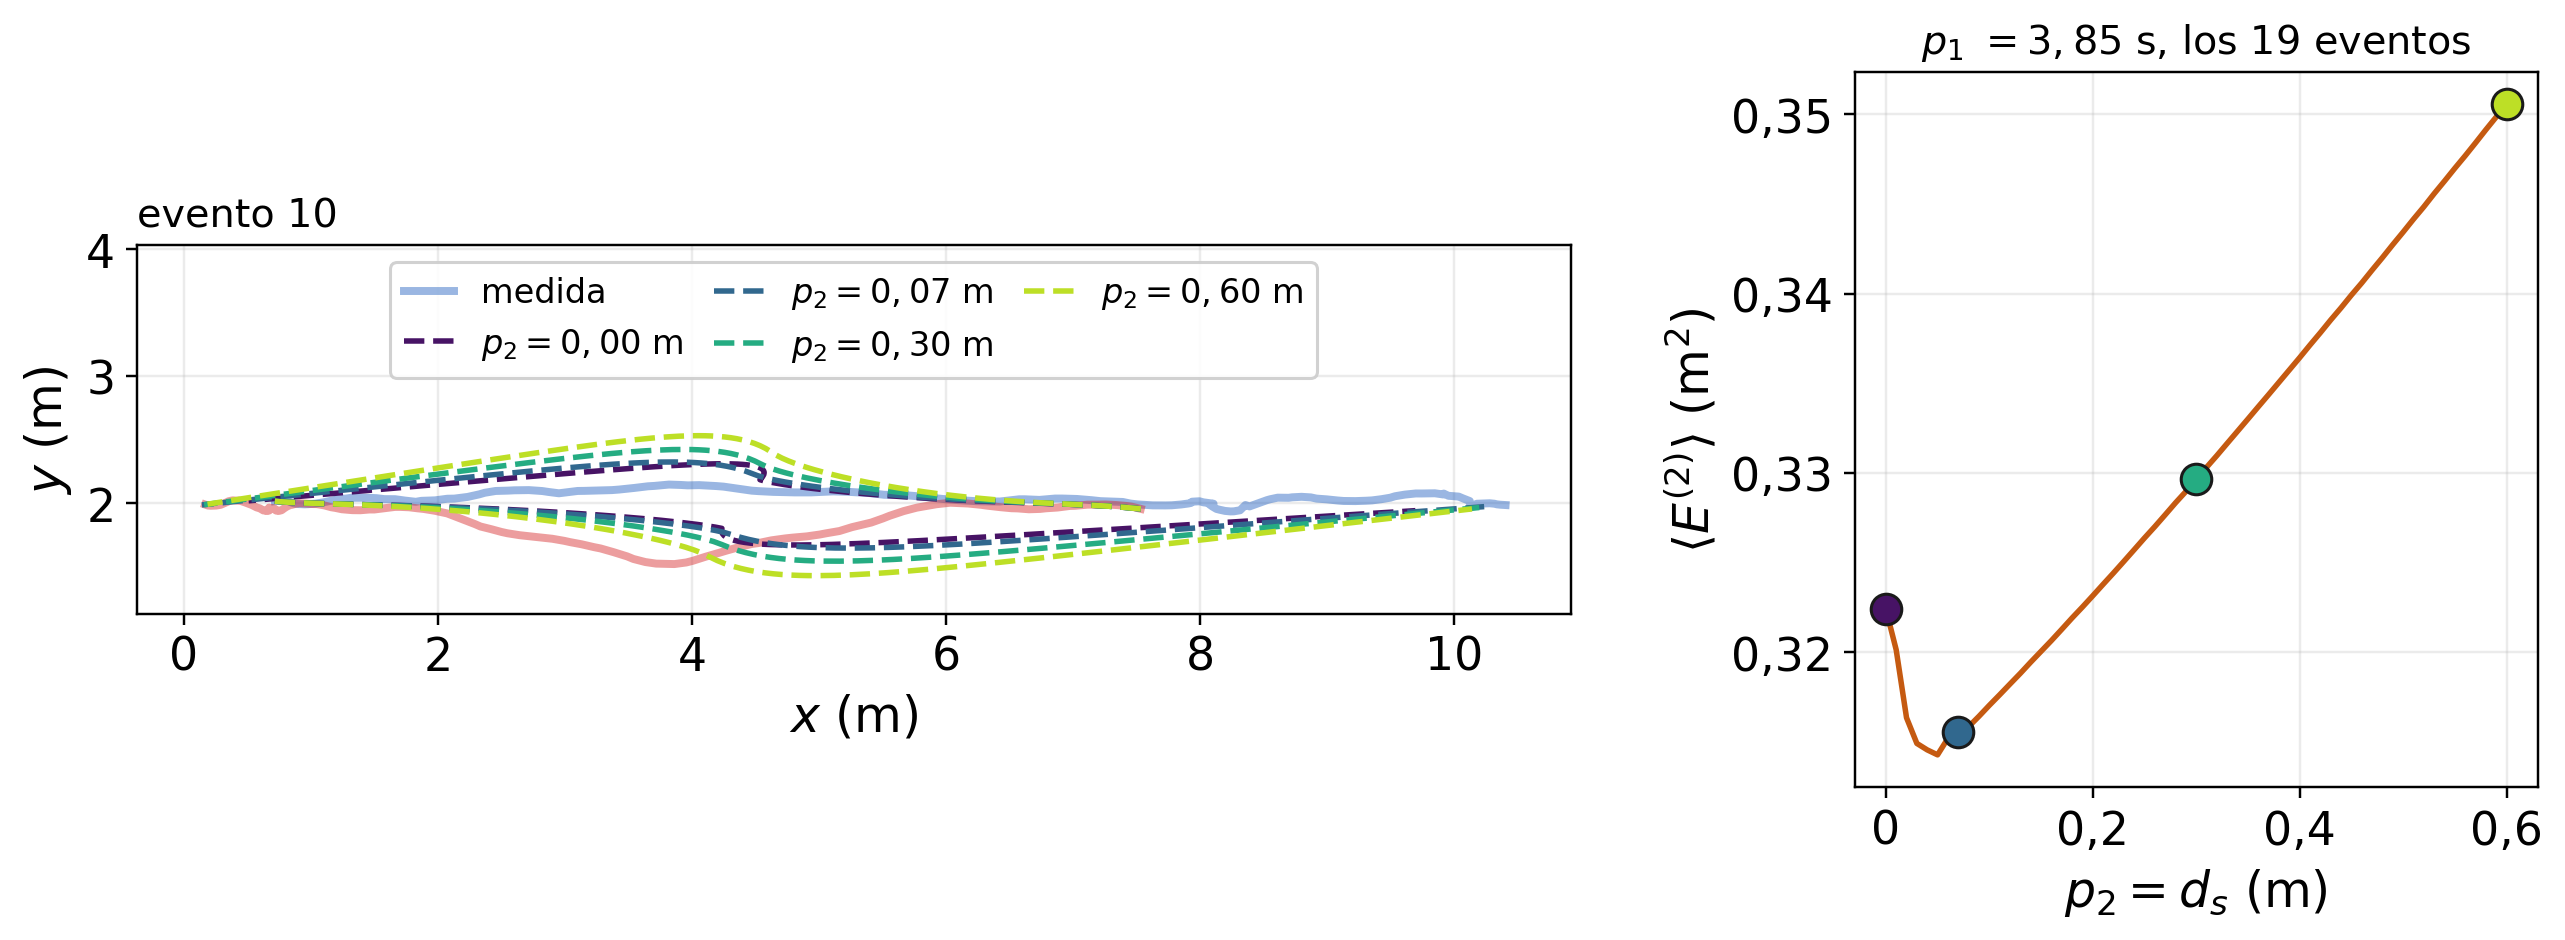
\includegraphics[width=\linewidth,height=0.70\textheight,keepaspectratio]{slide-20-que-hace-p2.png}
        \end{column}\hfill
        \begin{column}{0.36\textwidth}
            \small
            \begin{itemize}\setlength{\itemsep}{0.25em}
                \item El evento 10 con $p_2$ recorriendo su rango; al lado, el
                      corte de \mEdos{} con el punto donde está.
                \item $p_2$ fija \textbf{por dónde se pasa}: con $0{,}07$ pasan
                      rozándose como las personas; con $0{,}3$ y $0{,}6$ se abren
                      de más y \mEdos{} sube.
                \item $p_1$ (animación aparte) decide \textbf{si llegan a
                      correrse}: con \SI{0.5}{\second} reaccionan tarde; desde
                      $\approx \SI{1.2}{\second}$ ya no cambia nada.
                \cond{$p_1 = \SI{3.85}{\second}$; $p_2 = 0$, $0{,}07$, $0{,}3$ y \SI{0.6}{\meter}, un punto por valor en el corte}
            \end{itemize}
        \end{column}
    \end{columns}
    \begin{center}\video{https://youtu.be/PENDIENTE-07}\quad\video{https://youtu.be/PENDIENTE-08}\end{center}
\end{frame}

\begin{frame}{Ítem b: \mEuno{} sobre la grilla de parámetros}
    \figbulw[0.45em]{slide-21-superficie-metrica1.png}{%
        \item El color va con escala de potencia y las curvas de nivel son
              múltiplos del mínimo: en escala lineal todo el valle queda del
              mismo tono.
        \item \alert{Óptimo en $p_1 = \SI{2.50}{\second}$,
              $p_2 = \SI{0.07}{\meter}$}, con
              $\mEuno = 1{,}48 \pm \SI{0.25}{\meter\squared}$ (RMS
              \SI{1.22}{\meter}); sin capa, \SI{2.73}{\meter\squared}:
              \textbf{la capa baja el error un \SI{46}{\percent}}.
        \item El velo blanco marca los pares que \textbf{empatan} con el
              óptimo: $p_1$ de $0{,}85$ a \SI{4}{\second} y $p_2$ de $0{,}05$ a
              \SI{0.42}{\meter}. Más allá de $p_1 = \SI{4}{\second}$ nada cambia:
              hasta \SI{8}{\second} la diferencia pareada es $0{,}05 \pm
              \SI{0.04}{\meter\squared}$.
        \cond{19 eventos, $81 \times 61$ pares, $\dt = \dtexp/64$}
    }
\end{frame}

\begin{frame}{Ítem b: cortes por el óptimo, métrica 1}
    \figancha[0.86]{slide-22-cortes-metrica1.png}{%
        \colvin{%
            \item $p_1$ \textbf{sólo queda determinado por abajo}: \mEuno{} cae
                  de $2{,}73$ a \SI{1.5}{\meter\squared} entre 0 y
                  \SI{1.2}{\second} y después es plano.
            \item Es físico: con más de un segundo el agente ya llega a correrse
                  lo que necesita, y adelantar la reacción no cambia por dónde
                  pasa.}
        \colvin{%
            \item $p_2$ sí tiene un mínimo claro en \SI{0.07}{\meter} y sube
                  monótono después: es el parámetro que fija por dónde pasa.
            \cond{barra: error estándar de la media entre los 19 eventos; franja verde: los valores que empatan con el óptimo}}
    }
\end{frame}

\begin{frame}{Ítem b: \mEdos{} sobre la grilla de parámetros}
    \figbulw[0.45em]{slide-23-superficie-metrica2.png}{%
        \item Mismo valle, \textbf{más profundo}: sin capa
              $\mEdos = \SI{0.84}{\meter\squared}$ y en el óptimo
              $0{,}314 \pm \SI{0.074}{\meter\squared}$ (RMS \SI{0.56}{\meter}),
              \alert{un \SI{63}{\percent} menos}.
        \item \alert{Óptimo en $p_1 = \SI{3.85}{\second}$,
              $p_2 = \SI{0.05}{\meter}$}; la región que empata es mucho más
              chica (129 pares contra 1482): sacando el tiempo de paso, la
              métrica determina mejor los parámetros. Hasta \SI{8}{\second} la
              diferencia pareada es $0{,}000 \pm \SI{0.007}{\meter\squared}$.
        \item Los dos óptimos piden casi la misma distancia de paso:
              $\Dreq = 0{,}57$ y \SI{0.55}{\meter}.
        \cond{19 eventos, $81 \times 61$ pares, $\dt = \dtexp/64$}
    }
\end{frame}

\begin{frame}{Ítem b: cortes de la métrica 2 y comparación de los óptimos}
    \figancha[0.86]{slide-24-cortes-metrica2.png}{%
        \colvin{%
            \item Los dos óptimos coinciden en $p_2$ ($0{,}07$ contra
                  \SI{0.05}{\meter}) y difieren en $p_1$ ($2{,}50$ contra
                  \SI{3.85}{\second}), que es el parámetro plano.
            \item \alert{Intercambiarlos cuesta menos del \SI{2}{\percent}} en
                  cualquiera de las dos métricas: eligen esencialmente la misma
                  capa.}
        \colvin{%
            \item La diferencia es estadísticamente significativa con el test
                  pareado --- las dos superficies se miden sobre los mismos 19
                  eventos --- pero \textbf{irrelevante en magnitud}.
            \cond{mismas 19 realizaciones; franja verde: los valores que empatan con el óptimo}}
    }
\end{frame}

\begin{frame}{Ítem c: óptimos individuales}
    \figbulw[0.45em]{slide-25-optimos-individuales.png}{%
        \item Cada punto es el par que minimiza el error de \textbf{ese} evento;
              la estrella es el poblacional.
        \item En $p_2$ están todos juntos: mediana \SI{0.05}{\meter}, y 15 de 19
              por debajo de \SI{0.1}{\meter}. En $p_1$ están \textbf{desparramados
              por todo el rango}, y 8 caen en el borde $p_1 = \SI{4}{\second}$:
              es lo que se espera de un parámetro cuya dirección es plana.
        \item \alert{4 de los 19 eligen $p_1 = 0$}: a esos eventos la capa no
              les sirve. Son los que las personas resolvieron de una manera que
              el modelo no reproduce.
        \cond{métrica 1, misma grilla de $81 \times 61$ pares}
    }
\end{frame}

\begin{frame}{Ítem c: cuánto se gana al individualizar}
    \figbulw[0.45em]{slide-26-errores-por-evento.png}{%
        \item Evento por evento, el error con los parámetros poblacionales y con
              los propios. \textbf{Los eventos son muy desparejos}: de $0{,}38$ a
              \SI{4.0}{\meter\squared} con los mismos parámetros.
        \item \alert{Individualizar baja \mEuno{} de $1{,}48$ a
              \SI{1.22}{\meter\squared}, un \SI{17}{\percent}} --- y con la
              métrica 2, de $0{,}314$ a $0{,}296$, apenas un
              \SI{6}{\percent}.
        \item Es poco para 19 pares de parámetros contra uno: el error no está
              en los parámetros, \textbf{está en lo que el modelo no describe}.
        \cond{métrica 1; con la métrica 2 la figura es la misma y la ganancia, un tercio}
    }
\end{frame}

\begin{frame}{De dónde viene el error (1/3): dos poblaciones de eventos}
    \figbulw[0.25em]{slide-27-dos-poblaciones.png}{%
        \item Se separan solos por el ángulo entre $\vv(0)$ y el camino nominal:
              menor que $32^\circ$ (los dos \textbf{ya en el corredor}, 10
              eventos) o mayor que $60^\circ$ (alguno \textbf{sale de la fila},
              9 eventos).
        \item \alert{\mEdos{}: $0{,}08$ contra \SI{0.57}{\meter\squared}}. En
              los de la fila la recta al target es la \textbf{ruta equivocada}, y
              eso lo fija el enunciado, no la capa.
        \item Calibrando sólo con los 10 del corredor: $(\SI{4.0}{\second},\
              \SI{0.07}{\meter})$ y $\mEdos = \SI{0.078}{\meter\squared}$ (RMS
              \SI{0.28}{\meter}), \textbf{un \SI{92}{\percent} menos que sin
              capa}; sólo con los 9 de la fila, un \SI{19}{\percent}.
        \cond{métrica 2 con su óptimo poblacional; con la métrica 1: $0{,}78$ contra \SI{2.25}{\meter\squared}}
    }
\end{frame}

\begin{frame}{Evento 14: los dos salen de la fila}
    \figancha{slide-28-animacion-evento14.png}{%
        \colvin{%
            \item Las personas caminan primero \textbf{por la fila}, hacia arriba,
                  y doblan al corredor en $y \approx \SI{2}{\meter}$: su distancia
                  no baja hasta los \SI{3.5}{\second}.
            \item Los agentes van derecho al target desde $t = 0$, en diagonal, y
                  se cruzan a los \SI{4.7}{\second}, con las personas aún a
                  \SI{5.6}{\meter}.}
        \colvin{%
            \item $\Euno_m = \SI{3.44}{\meter\squared}$, el segundo peor. La capa
                  no puede arreglarlo: la ruta no es suya.
            \cond{$p_1 = \SI{2.5}{\second}$, $p_2 = \SI{0.07}{\meter}$; congelada en el último instante en conflicto, $t = \SI{4.66}{\second}$}}
    }
    \begin{center}\video{https://youtu.be/PENDIENTE-04}\end{center}
\end{frame}

\begin{frame}{De dónde viene el error (2/3): ritmo y forma}
    \figbulw[0.4em]{slide-29-residuo-descomposicion.png}{%
        \item $\Euno_m$ abierto en la componente \textbf{a lo largo} del camino
              nominal y la \textbf{perpendicular}, agrupado por población.
        \item En el corredor, \alert{el \SI{88}{\percent} es longitudinal}: es
              \textbf{ritmo}, el agente camina a $v^d$ constante y la persona
              acelera y frena. La forma --- lo que la capa decide --- es el
              \SI{12}{\percent}.
        \item En la fila la componente longitudinal también lleva la \textbf{ruta}
              (\SI{73}{\percent}), y la perpendicular es cinco veces mayor que en
              el corredor.
        \cond{$p_1 = \SI{2.5}{\second}$, $p_2 = \SI{0.07}{\meter}$; cada grupo ordenado por $\Euno_m$}
    }
\end{frame}

\begin{frame}{De dónde viene el error (3/3): el lado por el que se eluden}
    \figbulw[0.2em]{slide-30-residuo-lado.png}{%
        \item Desvío lateral entre los dos peatones en el cruce, medido contra
              simulado. En el fondo rojo el modelo eludió \textbf{por el lado
              opuesto}.
        \item \alert{Acierta en 12 de 19}: 6 de 10 en el corredor y 6 de 9 en la
              fila. Los que acierta tienen $\mEuno = \SI{1.32}{\meter\squared}$; los
              otros, $1{,}75$.
        \item La capa decide el lado con las velocidades del momento, y de
              frente lo decide un corrimiento de centímetros. Las personas lo
              deciden antes: en 14 de 19 cruces pasaron \textbf{cada uno por su
              derecha}.
        \cond{$p_1 = \SI{2.5}{\second}$, $p_2 = \SI{0.07}{\meter}$; el simulado está acotado por \Dreq}
    }
\end{frame}

\begin{frame}{Evento 3: en el corredor, pero por el lado opuesto}
    \figancha{slide-31-animacion-evento03.png}{%
        \colvin{%
            \item Las personas se cruzaron con el de la izquierda por abajo
                  ($\Delta y = \SI{-0.57}{\meter}$); el modelo, al revés
                  ($+0{,}57$).
            \item La elusión en sí es la correcta: pasan a \SI{0.57}{\meter}
                  contra \SI{0.60}{\meter} medidos.}
        \colvin{%
            \item $\Edos_m = \SI{0.31}{\meter\squared}$, el mayor del corredor:
                  todo el error es \textbf{el lado}.
            \cond{$p_1 = \SI{2.5}{\second}$, $p_2 = \SI{0.07}{\meter}$; congelada en el último instante en conflicto, $t = \SI{3.60}{\second}$}}
    }
    \begin{center}\video{https://youtu.be/PENDIENTE-05}\end{center}
\end{frame}

\begin{frame}{Ítem d: validación cruzada}
    \figbulw[0.45em]{slide-32-validacion-error.png}{%
        \item 500 particiones al azar: se calibra con 13 eventos y se mide sobre
              los otros 6, que no se usaron para calibrar.
        \item \alert{El error de validación queda un \SI{5.2}{\percent} por
              encima del del ítem b} ($1{,}55$ contra
              \SI{1.48}{\meter\squared}); dejando uno afuera, un
              \SI{6.4}{\percent}. Con la métrica 2 la diferencia es del
              \SI{0.2}{\percent}.
        \item Con dos parámetros y 19 eventos \textbf{no hay sobreajuste}: lo
              calibrado sobre una parte vale para la otra.
        \cond{métrica 1, 500 particiones de 13/6; la distribución de validación es más ancha porque promedia 6 eventos y no 19}
    }
\end{frame}

\begin{frame}{Ítem d: qué par elige cada partición}
    \figbulw[0.45em]{slide-33-validacion-parametros.png}{%
        \item El par calibrado cambia de partición en partición: 52 pares
              distintos en 500 particiones, y el más frecuente aparece en el
              \SI{26}{\percent}.
        \item \alert{La dispersión está casi toda en $p_1$} (de $0{,}75$ a
              \SI{4}{\second}); $p_2$ se queda entre $0$ y
              \SI{0.6}{\meter} con mediana \SI{0.08}{\meter}.
        \item Es la misma conclusión que la región que empata del ítem b, medida
              de otra manera: $p_2$ está determinado y $p_1$ sólo por abajo.
        \cond{métrica 1, 500 particiones de 13/6; el tamaño del punto es cuántas particiones eligieron ese par}
    }
\end{frame}

% =========================================================
\section{Conclusiones}
% =========================================================

\begin{frame}{Conclusiones}
    \vspace{0.1em}
    \small
    \begin{itemize}\setlength{\itemsep}{0.55em}
        \item Una capa de elusión de \textbf{dos parámetros} que sólo reemplaza el
              target baja el error poblacional un \SI{46}{\percent} con la métrica
              1 ($2{,}73 \to \SI{1.48}{\meter\squared}$) y un \SI{63}{\percent} con
              la métrica 2 ($0{,}84 \to \SI{0.31}{\meter\squared}$).
        \item Los óptimos son $(\SI{2.50}{\second},\ \SI{0.07}{\meter})$ y
              $(\SI{3.85}{\second},\ \SI{0.05}{\meter})$: las dos métricas piden la
              \textbf{misma distancia de paso}, $\Dreq \approx \SI{0.56}{\meter}$, e
              intercambiarlos cuesta menos del \SI{2}{\percent}.
        \item $p_2$ queda bien determinado y \textbf{$p_1$ sólo por abajo}: con más
              de \SI{1.2}{\second} de anticipación la superficie es plana dentro del
              error pareado, hasta \SI{8}{\second}.
        \item Los eventos son \textbf{dos poblaciones}: en los 10 en que los dos ya
              caminan por el corredor, $\mEdos = \SI{0.08}{\meter\squared}$ y la capa
              baja el error un \SI{92}{\percent}; en los 9 que salen de la fila,
              $0{,}57$, porque la recta al target es la ruta equivocada.
        \item Individualizar los parámetros gana un \SI{17}{\percent} y un
              \SI{6}{\percent}: el error que queda no está en los parámetros. En el
              corredor es \textbf{ritmo} (\SI{88}{\percent}) y \textbf{el lado}, que
              el modelo acierta en 6 de 10.
        \item La validación cruzada da un error apenas un \SI{5.2}{\percent} mayor
              que el del ítem b (\SI{0.2}{\percent} con la métrica 2): con dos
              parámetros y 19 eventos \textbf{no hay sobreajuste}.
    \end{itemize}
\end{frame}

\begin{frame}{Uso de agentes de IA}
    \vfill
    \begin{center}
    \begin{minipage}{0.88\textwidth}
        \normalsize
        \begin{itemize}\setlength{\itemsep}{0.9em}
            \item \textbf{Agente y modelo}: Claude Code (Anthropic), modelos Claude
                  Opus~5 y Claude Fable~5.1.
            \item \textbf{En qué se usó}: asistencia en la programación del motor en
                  C++, de los \textit{scripts} de post-procesamiento en Python y del
                  código \LaTeX{} de estas diapositivas, y revisión de código.
            \item \textbf{En qué no se usó}: el diseño de la capa de elusión, las
                  decisiones de modelado (ventana de cada evento, esquema de
                  integración, criterio de compatibilidad entre pares), el análisis
                  de los resultados y las conclusiones son del grupo, a partir de las
                  Teóricas 5 a 7 y de la bibliografía de la cátedra.
            \item Todo lo generado se revisó y se verificó contra las figuras
                  mostradas.
        \end{itemize}
    \end{minipage}
    \end{center}
    \vfill
\end{frame}

\begin{frame}[plain,noframenumbering]
    \vfill
    \begin{center}
        {\Large\bfseries\color{azul} Muchas gracias}\\[0.6em]
        \textcolor{azul!30}{\rule{0.25\textwidth}{1pt}}
    \end{center}
    \vfill
\end{frame}

\end{document}
